
\documentclass[11pt]{article}

\usepackage{amsmath}
\usepackage[noae] {Sweave}
\usepackage{amscd}
\usepackage[tableposition=top]{caption}
\usepackage{ifthen}
\usepackage{color}

\usepackage[margin=0.75in]{geometry}              

\usepackage[bookmarksnumbered,bookmarksopen,colorlinks,citecolor=blue,linkcolor=blue]{hyperref}
\usepackage{natbib}

\begin{document}
\Sconcordance{concordance:Screening_biomarker_07142018.tex:Screening_biomarker_07142018.Rnw:%
1 102 1 1 40 2 1 1 6 1 2 5 1 1 3 3 0 1 1 3 0 1 2 1 1 1 3 3 0 1 1 3 0 1 %
2 1 1 1 3 3 0 1 1 3 0 2 2 4 0 2 2 4 0 1 2 58 1 1 50 2 1 1 85 1 2 242 1 %
1 19 2 1 1 4 1 2 480 1}


\title{On Cost-Effectiveness of Screening Using a Marker/Risk-model}
\author{Ionut Bebu and Hormuzd Katki}
%IDCRP\\
%\texttt{ibebu@idcrp.org}}
\maketitle
%\tableofcontents

\section{Introduction}
Consider the problem of screening for cancer when a marker/risk-model is available. Each individual has a marker value or a risk score derived using a risk-model and the patient's characteristics. Individuals with high marker values or high risk scores are then tested for cancer. The problem is to identify an optimal cutoff value above which an individual needs to be tested for cancer. Notice that the lower the cutoff for the screening test is, the more likely a cancer case is detected (higher effectiveness), but also the higher the number of negative tests (higher costs). 

\section{Main} 
Katki \cite{katki} proposed a new measure of evaluating the risk before and after incorporating the marker information\footnote{\href{http://analysistools.nci.nih.gov/biomarkerTools}{See the online MRS webtool.}}. The mean risk classification (MRS) measure they proposed measure is the average change in risk (postttest - pretest). Briefly, their approach is to quantify the value of marker $M$ to predict the outcome $D$ by $P(D+|M+) - P(D+)$ if $M+$, and by $P(D-|M-) - P(D-)$ if $M-$, which yields (on average)
\begin{eqnarray}\label{MRS}
MRS &=& [P(D+|M+) - P(D+)]\cdot P(M+) + [P(D-|M-) - P(D-)]\cdot P(M-)\\    \label{MRS2}
    &=& 2[P(D+,M+) - P(D+)\cdot P(M+)]\,. 
\end{eqnarray} 
Here $M+$ denotes the event $M\geq m_0$, for some cutoff value $m_0$, while $M-$ denotes the event $M< m_0$.

It follows from (\ref{MRS2}) that $MRS$ is simply twice the covariance of $D+$ and $M+$. Therefore $MRS$ is indeed a measure of association between the marker and the outcome, but it is not immediately clear how relevant it is if the goal is to find an optimal cutoff value $m_0$. 

Katki \cite{katki} further show that 
\begin{equation}\label{MRS_AUC}
MRS=2J\cdot \pi(1-\pi)=4(AUC-0.5)\cdot \pi(1-\pi)\,,
\end{equation}
where $\pi=P(D+)$ and $J$ is Youden's index. However, notice that $\pi$ does not depend on the marker $M$, so that all three measures $MRS$, $AUC$ and $J$ are equivalent when it comes to choosing the marker cutoff value $m_0$. 

Alternatively, one can introduce a cost-effectiveness framework for this problem as follows. Assume the effectiveness score for a subject who does not develop cancer is 1, and let $e_1$ denote the effectiveness score for a subject with a positive marker $M$ which then tests positive for cancer; similarly, let $e_2$ be the effectiveness score for subject who is either not screened using the marker $M$ or is $M-$, but then develops cancer. Since the cancer cases identified using the marker $M+$ are diagnosed earlier, it follows that $e_1 > e_2$, and both are less than 1. 

Let $c_m$ denote the cost of a marker evaluation, $c_0$ denote the cost of standard test for cancer, $c_1$ the cost of treatment for a cancer case diagnosed early (i.e., tested positive for $M$), and $c_2$ the treatment cost for a cancer case diagnosed late (i.e., either not screened with $M$ or tested negative for $M$). 

Two scenarios are considered at individual level:
\begin{enumerate}
   \item{No screening for $M$. There are two possibilities:
     \begin{enumerate}
        \item{The individual has cancer ($D+$): cost is $c_0+c_2$ and effectiveness is $e_2$}
        \item{The individual does not have cancer ($D-$): cost is 0, effectiveness is 1.}
     \end{enumerate}
   }
   \item{Screening for $M$. There are four possibilities:
      \begin{enumerate}
        \item{The screening is positive and the individual has cancer ($M+,D+$): cost is $c_m+c_0+c_1$and effectiveness is $e_1$.}
        \item{The screening is positive but the individual does not have cancer ($M+,D-$): cost is $c_m+c_0$and effectiveness is $1$.}
        \item{The screening is negative but the individual has cancer ($M-,D+$): cost is $c_m+c_0+c_2$and effectiveness is $e_2$.}
        \item{The screening is negative and the individual has not have cancer ($M-,D-$): cost is $c_m$and effectiveness is $1$.}
      \end{enumerate}  
   }
\end{enumerate}

Let $C$ and $E$ denote the cost and effectiveness without screening, and $C_M$ and $E_M$ with screening. One has
\begin{eqnarray*}
{\cal E} (C) &=& (c_0+c_2)\cdot P(D+) \\
{\cal E} (E) &=& e_2\cdot P(D+) + P(D-) \\
{\cal E} (C_M) &=& c_m + [1-P(D-,M-)]\cdot c_0+P(D+,M-)\cdot c_2+P(D+,M+)\cdot c_1\\
{\cal E} (E_M) &=& P(D-) + P(D+,M+)\cdot e_1 + P(D+,M-)\cdot e_2 \,,
\end{eqnarray*}
so that the differences in cost and effectiveness between the two scenarios are 
\begin{eqnarray*}
\Delta C &=& c_m + c_0\cdot P(M+) + (c_1 - c_2 - c_0)\cdot P(D+,M+)\\
\Delta E &=& (e_1 - e_2)\cdot P(D+,M+)\,.
\end{eqnarray*}
One then selects $m_0$ based on both $\Delta C$ and $\Delta E$. Notice that $\Delta E$ is maximized when $m_0=-\infty$ (i.e., screen everybody). 

\section{Illustration}

Let $\tilde{M}$ such that the true risk of cancer is
\begin{equation}\label{model_D}
P(D=1|\tilde{M}=\tilde{m})=L(\alpha_0 + \alpha_1\cdot \tilde{m})\,,
\end{equation} 
where $L(x)=\exp(x)/(1+\exp(x))$.

However, $\tilde{M}$ is not directly observed. Instead, one observes a marker $M$, where
\begin{equation}\label{model_M}
M = \tilde{M} + \epsilon\,.
\end{equation}
We further assume $\epsilon\sim N(0,\sigma_\epsilon^2)$, and $M\sim N(\mu_M,\sigma_M^2)$. One obtains
\begin{eqnarray*}
P(M+) &=& 1-\Phi\left(m_0-\mu_M,0,\sigma_M^2 +\sigma_\epsilon^2 \right)   \\
P(D+,M+) &=& \int_{m_0}^\infty \int_{\infty}^{\infty}L(\alpha_0+\alpha_1\cdot(m-\epsilon))\cdot \phi(\epsilon,0,\sigma_\epsilon^2)
  \cdot \phi(m,\mu_M,\sigma_M^2)d\epsilon \, dm
\end{eqnarray*}
while $P(D+)$ is obtain by replacing $m_0$ by $\infty$ in the expression for $P(D+,M+)$ above. 

The approaches are illustrated using $\alpha_0 = -6.67$, $\alpha_1 = 1$,
$\mu_M = 1$, $\sigma_M=1$, $c_m=0.5$, $c_0=0.01$, $c_1=1$ and $c_2=2$.


\begin{figure}
\begin{center}
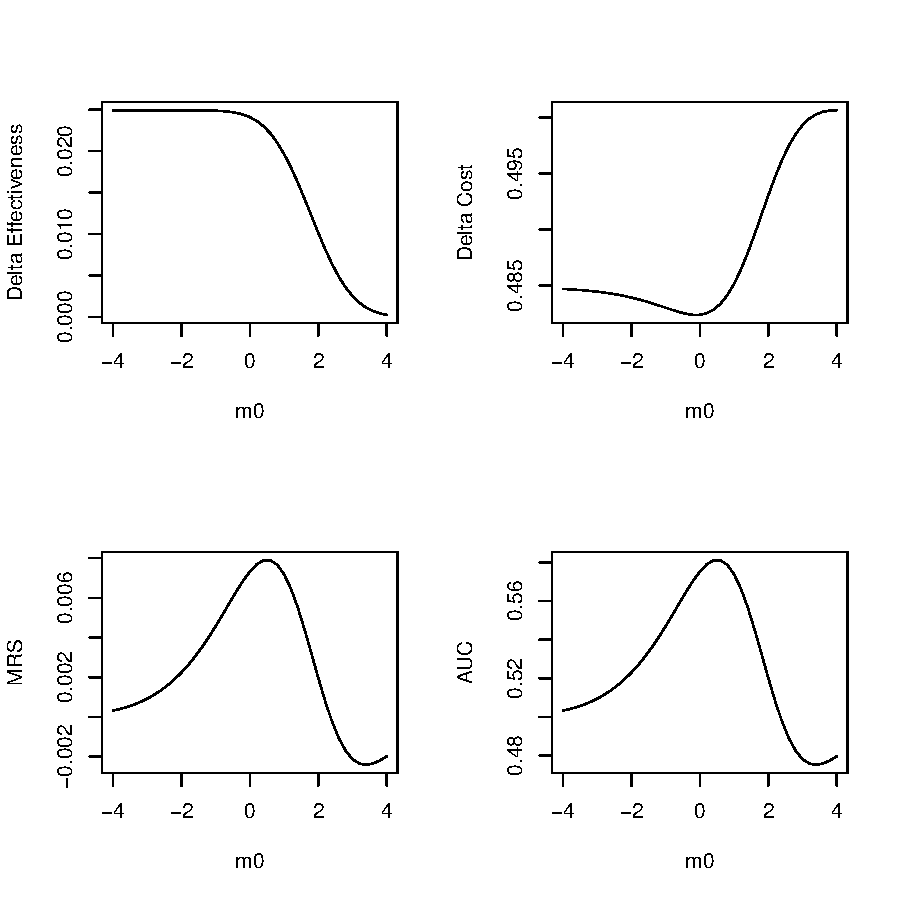
\includegraphics{Screening_biomarker_07142018-fig1}
\end{center}
\label{fig:one}
\caption{Effectiveness, cost, MRS and AUC as a function of the cutoff value $m_0$.}
\end{figure}

The optimal $m_0$ with respect to the ICER (i.e., lowest ICER) and the corresponding ICER are
\begin{Schunk}
\begin{Soutput}
[1] -1.4
\end{Soutput}
\begin{Soutput}
[1] 19.39465
\end{Soutput}
\end{Schunk}

The optimal $m_0$ with respect to the AUC (i.e., largest AUC) and the corresponding ICER are
\begin{Schunk}
\begin{Soutput}
[1] 0.6
\end{Soutput}
\begin{Soutput}
[1] 0.5811674
\end{Soutput}
\end{Schunk}

The optimal $m_0$ with respect to the MRS (i.e., largest MRS) and the corresponding ICER are
\begin{Schunk}
\begin{Soutput}
[1] 0.6
\end{Soutput}
\begin{Soutput}
[1] 0.00789477
\end{Soutput}
\end{Schunk}
As expected, MRS and AUC give identical results, but which are different than the ones for ICER. Moreover, the $m_0$ value selected by MRS/AUC has an ICER value of 
\begin{Schunk}
\begin{Soutput}
[1] 21.83748
\end{Soutput}
\end{Schunk}
or a 
\begin{Schunk}
\begin{Soutput}
[1] 11.18642
\end{Soutput}
\end{Schunk}
percent (\%) increase relative to the optimal ICER.

%<<time>>=
%Sys.time() - tt
%@

\section{Discussion}

Various approaches for calculating an optimal cutoff for a screening marker were considered. The MRS measure, which is twice the covariance between $D+$ and $M+$ is shown to be equivalent to AUC with respect to selecting this optimal cutoff $m_0$. 

Note that the above calculations depend on the unobserved $\alpha_0$, $\alpha_1$ and $\sigma_\epsilon$. However, for various values of $\sigma_\epsilon$, one can estimate $\alpha_0$ and $\alpha_1$ based on the coefficients obtained by regressing $D=1$ on $M$, which can then be used to find the optimal cutoff value $m_0$. 



\section{Incremental Net Benefit}

A large Incremental Cost-Effectiveness Ratio (ICER) can mask a small difference, and vice-versa.  For this reason, the Incremental Net Benefit (INB) is better:
\begin{eqnarray*}
INB &=& \Delta E - \Delta C.
\end{eqnarray*}
This requires redefining Effectiveness as the dollar value of each life-year gained.

\subsection{Application to deciding who should undergo \textit{BRCA1/2} genetic testing}

We previously applied MRS to the controversy over who should get tested for mutations in the \textit{BRCA1/2} genes, which cause high risks of breast and ovarian cancer~\citep{katki}.  The mutations are rare in the general population ($\approx0.25\%$), but are 10 times more common among Ashkenazi-Jews~\citep{STRUEWING1997}.  Currently, according to the UK National Institute for Health and Care Excellence (NICE) and the US Preventive Services Task Force, women are referred for mutation testing only if they have a strong family history of breast or ovarian cancer~\citep{Moyer2014} as quantified by a risk model calculating that their risk of carrying a mutation exceeds 10\%~\citep{NICE2017}.  However, as mutation-testing costs fall, prominent voices have called for testing \textit{all} women~\citep{King2014,GenomeWeb2017}.  \textit{BRCA1/2} testing is already being offered to a large unselected Canadian population as a demonstration project~\citep{GenomeWeb2017a}.  Testing all women would strain clinical resources by testing millions of women, $99.75\%$ of whom will test negative.  At US \$500-\$1,000 per test, testing millions of women has clear commercial implications.  

In contrast, we recently demonstrated that 80\% of Ashkenazi-Jewish mutation-carriers could be identified by testing only 44\% of Ashkenazi-Jewish women~\citep{Best2017}.  This is achieved by a low mutation-risk threshold of 0.78\%, far lower than the current 10\% UK NICE and US recommendation.   However, we could not formally justify any choice of risk-threshold.  To better understand the implications of different choices of risk threshold, we previously considered multiple metrics, including AUC, Net Benefit, and MRS/NBI \citep{katki}.  We showed that risk thresholds between 0.78\% to 5.0\% maximized the MRS ($\approx 1.7\%$) for Ashkenazi-Jewish women, and for the general population, thresholds between 0.07\% to 0.56\% maximized the MRS ($\approx 0.18\%$)~\citep{katki}.  Here we compare risk thresholds that maximize MRS to risk thresholds that maximize the INB.

We use data on 4,589 volunteers (102 \textit{BRCA1/2} mutation carriers) from the Washington Ashkenazi Study (WAS)~\citep{STRUEWING1997}.  We calculated each volunteer's risk of carrying a mutation, based on their self-reported family-history of breast/ovarian cancers, using the BRCAPRO risk model~\citep{Parmigiani1998}.  Here $M$ is the BRCAPRO risk score, and because BRCAPRO is a well-calibrated risk model~\citep{Best2017}, $m_0=R$, i.e. the cutpoint $m_0$ equals the risk threshold $R$. Disease $D$ indicates the presence of a \textit{BRCA1/2} mutation.

\subsection{Costs and Effectiveness of \textit{BRCA1/2} genetic testing, preventive interventions, and cancer treatments}

Let us redefine Effectiveness as the dollar value of the life-years gained by undergoing genetic testing.  Let us presume that  women without mutations have a normal lifespan of age 80.  \textit{BRCA1/2} mutation-carriers have 5.7 fewer years of expected life~\citep{mai}, so we set their life-expectancy to age 74.  

If mutation-carriers get genetic testing, they will act to reduce their cancer risks.  Most mutation-carriers undergo oophorectomy, the removal of ovaries.  Some also choose to have mastectomy, the removal of breasts.  These surgeries reduce cancer risk drastically, but not entirely; there is typically a 10\% chance that cancer occurs in each organ anyway.  These women also undergo frequent screening, and if cancer is found early, hopefully treatment is more effective.  I don't know what their life-expectancy is, but let me set it as age 78.

I set the dollar-value of each life-year gained as \$100,000 per year.  Thus Effectiveness is
\begin{eqnarray*}
e_1-e_2 &=& (78-74)\times\$100,000 = \$400,000
\end{eqnarray*}

For costs, $c_m$ is the cost of using the BRCAPRO risk model.  This is very low-cost, but you need to come to the doctor's office, your family history has to be elicited, it takes time.  I will set it to the cost of a doctor's visit, say \$100.

$c_0$ is the cost of the BRCA genetic test.  Prices are falling, it is now about \$1,000.

$c_1$ is the cost of interventions for BRCA mutation carrier found by screening.  Generally they will undergo risk-reducting interventions, at least oophorectomy and perhaps also mastectomy, and then frequent lifetime cancer screening.  But cancer can still occur, and those 25\% (\textcolor{blue}{\it should this be related to the 10\% mentioned above?}) who still get cancer incur cancer treatment costs.  For $c_2$, this is the cost of cancer treatment for mutation carriers who are not found until cancer is diagnosed.  All of them will require full cancer treatment.  I don't know how to specify $c_1,c_2$.  Let me set them both equal to \$100,000 for now.

Thus we have for Costs:
\begin{eqnarray*}
  c_m &=& \$100 \\
  c_0 &=& \$1,000 \\
  c_1 &=& \$100,000 \\
  c_2 &=& \$100,000. \\
\end{eqnarray*}

%At a future time, it may be worth decomposing $c_1$ into the cost for the risk-reducing interventions that everyone

\subsection{MRS vs. INB for \textit{BRCA1/2} genetic testing}


\begin{figure}
\begin{center}
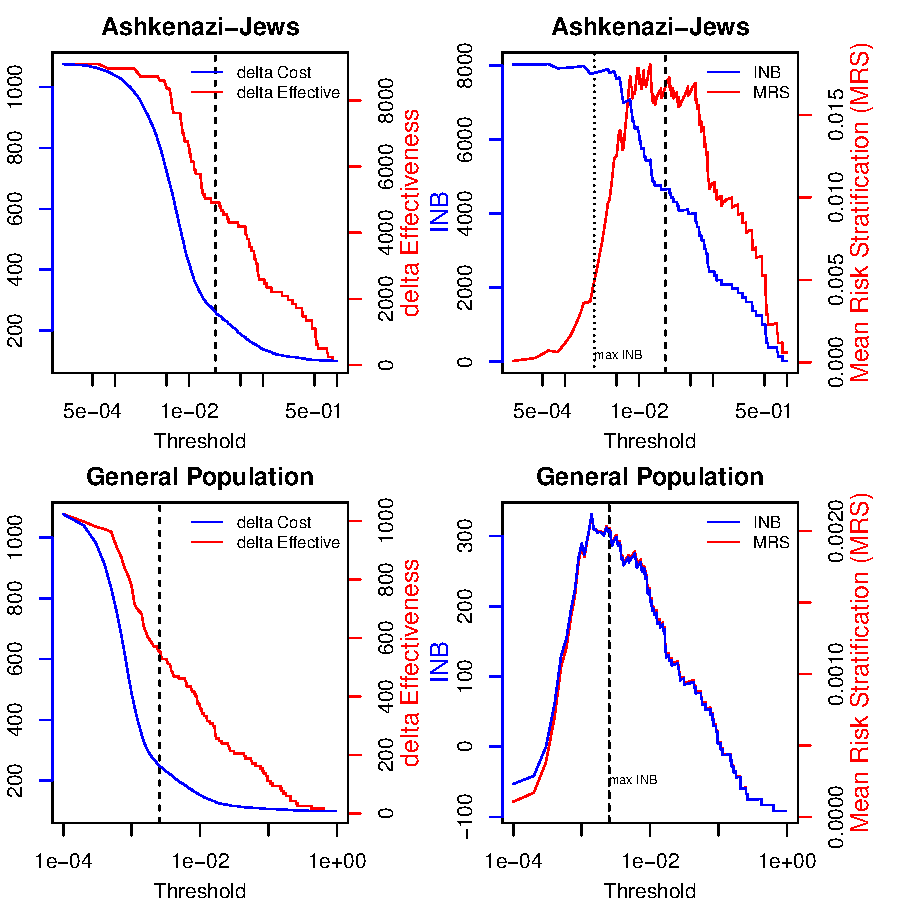
\includegraphics{Screening_biomarker_07142018-MRS_INB}
\end{center}
\label{fig:two}
\caption{Effectiveness, cost, MRS and INB as a function of the cutoff Threshold values $m_0$.  The marker is the BRCAPRO model score (cutoff at thresholds $m_0$), the confirmatory test is the BRCA genetic test itself.  The outcome $D+$ is having a BRCA mutation.  Costs $c_1$ and $c_2$ include risk-reducing interventions for the found BRCA mutation carriers, and cost of future cancer treatments. Effectiveness is the dollar value of the the life-years gained by early intervention.  First row is for Ashkenazi-Jews, second row is for general population.  Dashed line is where threshold equals mutation prevalence (2.3\% for Ashkenazi-Jews, 0.26\% for general population).  Dotted line is the risk threshold that maximizes INB which is $\pi_{INB}$}
\end{figure}

Figure 2 (left panels) show the increase in effectiveness and costs due to genetic testing for both Ashkenazi-Jews and the general population, as a function of the BRCAPRO risk threshold to offer women genetic testing.  When the threshold is low, most everyone is offered testing.  The cost is highest here, and decreases down to only marker testing cost (i.e. BRCAPRO risk model cost) if no one is offered genetic testing.  Effectiveness is also highest if everyone is tested for mutations, and goes down to zero if no one is.  Note that while the cost scale (y-axes) are the same, the effectiveness scale (right-axes) is about 10 times higher for Ashkenazi-Jews.  This reflects that mutations are 10 times more common for Ashkenazi-Jews.  

(Parenthetically, note that in the limits of testing no one or testing everyone, I should subtract out marker cost $c_m$ because the marker is unnecessary.  The limits of the INB curve don't equal the correct limits.  I should probably add two points on the figures for the INBs of testing everyone or no one.)

Figure 2 (right panels) compare the MRS to INB.  MRS is zero if no one, or everyone, gets mutation testing, and always peaks at threshold equals prevalence (dotted line).  INB for Ashkenazi-Jews is highest at a threshold of zero, meaning everyone should get testing  This happens because the of the high value attached to each life-year gained, and Ashkenazi-Jews are much more likely to gain this benefit.  For the general population, note that $INB<0$ for the lowest risk thresholds and for risk thresholds greater than 10\% (recall that 10\% is the current official threshold in the US and UK.).  These are thresholds where net harm would be done to the population.  

Importantly, for the general population, the INB curve is proportional to the MRS curve (i.e. the curves overlap, but note the very different scales on the left-axis and right-axis).  Thus INB and MRS are maximized at the same risk-threshold and give the same answer.  The next section shows that this happens because the costs and effectiveness balance each other in a special way.


\subsection{Example: single CT lung-cancer screen}

The eligible population for lung-cancer screening is you must be ages 55-80, smoked at least 30 pack-years, and cannot have quit for more than 15 years.  We will assume this population is fixed, as all the data is based on this population anyway.  The question is then, what is the cost-effectiveness of a single CT lung-cancer screen.

To estimate effectiveness, we need to know the the life-expectancy in this population, with and without a single screen.  $e_1$ is the number of life-expectancy for someone whose cancer is detected by CT and $e_2$ is the life-expectancy if the cancer is not detected by CT (in dollar value). Without dollar value, the years-gained by Bill Black's NEJM paper is roughly $e_1-e_2=8.4792-6.8479=1.6313$.  That is for 3 screens, let's assume for 1 screen we can divide by 3, so the life-years gained is 0.54377.  At \$100,000 value per life year, this is
\begin{eqnarray*}
e_1-e_2 &=& 0.54377\times\$100,000 = \$54,377
\end{eqnarray*}

% This is wrong: effectiveness e_1 is life-years gained for someone with early-detected cancer
% We have developed a calculator for life-expectancy gain for ever-smokers from a 3-screen program.  
% We estimate the life-gained to be an average of 16.2 days over your lifetime.  This is a typically pathetic benefit of cancer screening.  But that is for 3 screens, perhaps for 1 screen we can divide by 3 so we have something like 5.4 extra days of life from a single CT screen.  Setting the dollar-value of each life-year gained as \$100,000 per year (\$274 per day), effectiveness is
% \begin{eqnarray*}
% e_1-e_2 &=& 5.4\times\$274 = \$1,480
% \end{eqnarray*}
% (Note for Hormuzd:  Bill Black's paper estimates life-days gained in NLST as $(14.7386-14.7071)*365=11.5$ days.)

For costs, $c_m$ is the cost of a CT screen.  By Bill Black's NEJM paper, the screen is \$1,130 and work-up is \$835 for a total of $c_m=\$1,965$.

$c_0$ is the cost of the definitivly diagnosing lung cancer.  If this is a bronchoscopy with biopsy, Bill Black's paper gives lots of costs for different ways to do this, but this is about \$500.

$c_1$ is the cost of treating lung cancer found during screening and $c_2$ is the cost of treating lung cancer when there is no screening.  By Bill Black's paper, it looks like treatment cost under screening is $c_1=\$8,461$ and for no screening $c_2=\$7,835$, so $c_1-c_2=\$625$  (Note for Hormuzd: These treatment costs seem way too low.)

% Treatment costs estimate from Bill Black's paper
% I think Bill Black's treatment cost estimate of $1106 and $931 in table 2 is per the whole 53502 cohort.
% I'm not sure how to get this down to a treatment cost per cancer for CT vs. CXR.
% CT arm:  Total costs over trial (6.5 years/person) per year is $1106*53502/6.5 then divide by 1076 cancers for cost/cancer
% > 1106*53502/1076/6.5
% [1] 8460.568
% CXR arm:  Total costs over trial (6.5 years/person) per year is $931*53502/6.5 then divide by 978 cancers for cost/cancer
% > 931*53502/978/6.5
% [1] 7835.514
% Thus c_1=$8461 and c_2=$7836, difference of $625

Thus we have for Costs:
\begin{eqnarray*}
  c_m &=& \$1,965 \\
  c_0 &=& \$500 \\
  c_1 &=& \$8,461 \\
  c_2 &=& \$7,835. \\
\end{eqnarray*}

Thus $e=(e_1-e_2)-(c_1-c_2-c_0)=\$54,377-(\$625-\$500)=\$54,227$.  The optimal risk-threshold for a CT screen is $\pi_{INB}=c_0/(e+c_0)=0.91\%$ lung-cancer risk.  In comparison, by the Church NEJM paper, the 1st screen PPV  was 3.8\%, so the implicit NLST risk threshold was even lower than 3.8\%.  Perhaps it could be around 0.91\%, since average risk is probably much bigger than the minimum risk threshold. 

The INB is $eP(D+,M+)-c_m-c_0P(M+)$.  The Church NEJM paper reports $P(M+)=27.3\%$, $P(D+)=1.1\%$, and I calculate $P(D+,M+)=1.028\%$.  The INB is -\$1,543, which would mean screening should never be done.

Note that $INB>0$ iff $eP(D+,M+)>c_m+c_0P(M+)=\$2,102$ and thus $e>\$204,426$.  Given the costs as I understand them, there is no way a single CT screen can be cost-effective.


\section{When is INB proportional to MRS, so they have the same maximum?}

\begin{eqnarray*}
  INB &=& \Delta E - \Delta C\\
      &=& [(e_1-e_2)-(c_1-c_2-c_0)]P(D+,M+) - c_m - c_0P(M+).
\end{eqnarray*}
Define $p=P(M+)$ and $\pi=P(D+)$.  Recall that $P(D+,M+) = MRS/2 +p\pi$.  Define the net effectiveness of early intervention: $e = (e_1-e_2)-(c_1-c_2)$.  Then
\begin{eqnarray*}
  INB &=& (e+c_0)[MRS/2 + p\pi] - c_m - c_0p \\
      &=& (e+c_0)MRS/2 - c_m + p[e\pi + c_0\pi - c_0] \\
      &=& (e+c_0)MRS/2 - c_m + p[e\pi - c_0(1-\pi)].
\end{eqnarray*}
Note that $INB\propto MRS$ if $e\pi - c_0(1-\pi)=0$, which happens when
\begin{eqnarray*}
  \frac{\pi}{1-\pi} &=& \frac{c_0}{e} = \frac{c_0}{(e_1-e_2)-(c_1-c_2)},~~or~~\pi_{INB}=\frac{c_0}{c_0+e}.
\end{eqnarray*}
INB and MRS will have the same maximum if the odds of disease equals the ratio of confirmatory test cost to the net effectiveness of early intervention.  Let us call this critical prevalence $\pi_{INB}$ to indicate that this is the disease prevalence where MRS and INB yield the same optimal threshold.  In Figure 2, $c_0/e = \$1,000/(\$400,000-\$0) = 0.25\%$, and thus the critical prevalence is $\pi_{INB}=0.25\%$.  For the general population, $\pi=0.26\%$, which is very close to the critical prevalence.  

There is no reason for the confirmatory test cost and net effectiveness to balance in a way that their ratio equals the prevalence odds.  However, it is useful to calculate the critical prevalence and compare to the observed disease prevalence, to qualitatively understand which way the threshold for maximum MRS changes when costs and effectiveness are accounted for.  For example, for Ashkenazi-Jews, the prevalence is much higher than the critical prevalence ($2.5\% > 0.25\%$).  Thus immediately you know that the optimal threshold will decrease from prevalence towards testing more women than MRS would indicate.  



\section{Optimal cutoff threshold to maximize Incremental Net Benefit (INB)}

Recall that the optimal threshold to maximize MRS is the same as that for Youden's index, which is risk threshold equals prevalence~\citep{katki}, see Appendix.

Here I derive the optimal threshold that maximizes INB.  Recall that 
\begin{eqnarray*}
  INB &=& (e+c_0)MRS/2 - c_m + p[e\pi - c_0(1-\pi)]~=~(e+c_0)MRS/2 - c_m + p[\pi(e+c_0) - c_0].
\end{eqnarray*}
INB increases as MRS increases, but the last term decreases INB as $p=P(M+)$ increases.  To find the optimal threshold, let's find a simpler function with the same maximum  Dividing both sides by the constant $e+c_0$ yields
\begin{eqnarray*}
  \frac{INB}{e+c_0} &=& MRS/2 - \frac{c_m}{e+c_0} + p[\pi - \pi_{INB}].
\end{eqnarray*}
Because $MRS=2J\pi(1-\pi)$, then dividing by the constant $\pi(1-\pi)$ yields
\begin{eqnarray*}
  \frac{INB}{(e+c_0)\pi(1-\pi)} &=& J - \frac{c_m}{(e+c_0)\pi(1-\pi)} + p\frac{\pi - \pi_{INB}}{\pi(1-\pi)}.
\end{eqnarray*}
Explicitly writing INB, $J$, and $p$ as functions of cutoff thresholds $m_0$,
\begin{eqnarray*}
  INB(m_0) &\propto& J(m_0) + p(m_0)c,
\end{eqnarray*}
where $c=\frac{\pi - \pi_{INB}}{\pi(1-\pi)}$.  This is a simpler function to optimize.  Following the Appendix, we optimize by
differentiating $J(m_0)+p(m_0)c$ 
\begin{eqnarray*}
	J(m_0)+p(m_0)c &=& \int_{m_0}^\infty P(M=m|D+)-P(M=m|D-)+cP(M=m)~dm
\end{eqnarray*}
with respect to the cutpoint $m_0$ using the Leibniz Integral Rule:
\begin{eqnarray*}
	\frac{d(J(m_0)+p(m_0)c)}{dm_0} &=& P(M=m_0|D-)-P(M=m_0|D+)-cP(M=m_0).
\end{eqnarray*}
Setting the derivative equal to zero, and using Bayes' rule:
\begin{eqnarray*}
  cP(M=m_0)+\frac{P(D+|M=m_0)P(M=m_0)}{\pi} &=& \frac{P(D-|M=m_0)P(M=m_0)}{1-\pi}.
\end{eqnarray*}
Note that the risk threshold is defined as $R(m_0)=P(D+|M=m_0)$.  Note that $R(m_0)=m_0$ because $M$ is a risk-model.  Canceling $P(M=m_0)$, 
\begin{eqnarray*}
	\frac{c\pi+R}{\pi} &=& \frac{1-R}{1-\pi}\\
	\pi(1-R) &=& (c\pi+R)(1-\pi)\\
	\pi(1-R) &=& c\pi(1-\pi) + R(1-\pi)\\
	R &=& \pi - c\pi(1-\pi)~=~ \pi - (\pi-\pi_{INB})~=~\pi_{INB}
\end{eqnarray*}
Thus INB is maximized at risk threshold $R=\pi_{INB}=c_0/(e+c_0)$.

Note that $\pi_{INB}$ only requires the utilities: genetic test cost $c_0$ and the net effectiveness of early intervention $e=(e_1-e_2)-(c_1-c_2)$.  None of the objective aspects of the problem matter, like disease prevalence, etc.  This is unlike MRS, Youden's index, AUC, Vickers's Net Benefit gain, which are all maximized at risk threshold equals disease prevalence, regardless of your utilities.

Note that $\pi_{INB}$ doesn't require the marker cost $c_m$.  Thus you don't need to specify $c_m$ to find the optimal risk threshold.  Because $c_m$ contributes to the INB level, we only need it to make sure that the INB is greater than the INBs for testing no one or testing everyone.

Figure 2, dotted line, is the optimal risk threshold cutoff for INB, $R=\pi_{INB}=0.25\%$.  For the general population, this coincides with disease prevalence, and thus $INB\propto MRS$ so they are maximized at the same risk threshold.  For Ashkenazi-Jews, $R=\pi_{INB}=0.25\%$ is to left of prevalence $\pi=2.5\%$, which tests 85\% of Ashkenazi-Jews to find 96\% of BRCA mutation carriers.  The INB at 0.25\% is about \$7,800. INB for testing everyone is $INB_{all}=\$8,119$, which of course removes the \$100 cost of doing the marker, which is the BRCAPRO risk model.  For Ashkenazi-Jews, INB is maximixed where everyone gets genetic testing for BRCA mutations, regardless of BRCAPRO risk score.

If we halve the dollar value of each life-year gained from \$100,000 to \$50,000, then the optimal risk-threshold doubles to $\pi_{INB}=0.50\%$.  For the general-population, the $INB>0$ for risk threshlds from 0.17\%-1.87\% and the peak is indeed roughly at 0.50\% (INB=\$33.94, barely positive).  For Ashkenazi-Jews, the interior peak is at 0.50\%, but testing everyone still has a slightly higher INB.  

If we further halve the dollar value of each life-year gained to \$25,000, then the optimal risk-threshold doubles to $\pi_{INB}=0.99\%$.  For the general-population, all $INB<0$, the least bad INB is for testing no one (this is a case where we can only minimize harm, there are no good options).  For Ashkenazi-Jews, $INB>0$ for risk-thresholds of 0\%-5\%, and the peak is around 0.99\% (INB=\$1,235), although numerically 0.54\% has best INB=\$1,400.

Ionut, why don't you calculate INB and the optimal $\pi_{INB}$ for your logistic regression example?

\section{Conditions for a marker to have greater INB than another marker}

If one marker has greater sensitivity but less test positivity (or greater specificity yet more test positivity), then it is obviously that the marker is better, no cost-effectivenss analysis is needed.  However, there is usually a tradeoff, one test having better sensitivity but not specificity.  The tradeoff should be evaluated based on INB.

For two markers $\Delta INB=INB_1-INB_2>0$ if
\begin{eqnarray*}
\Delta INB &=& (e+c_0)[P(D+,M_1+)-P(D+,M_2+)] - c_0[P(M_1+)-P(M_2+)]\\
           &=& (e+c_0)[Sens_1-Sens_2]\pi - c_0[p_1-p_2] > 0
\end{eqnarray*}
for disease prevalence $P(D+)=\pi$ and test-positivities $p_1,p_2$.  Presuming $p_1>p_2$,
\begin{eqnarray}
\frac{Sens_1-Sens_2}{p_1-p_2} &>& \frac{c_0/[e+c_0]}{\pi} = \frac{\pi_{INB}}{\pi},
\end{eqnarray}
A usable test requires that the ratio of the the sensitivity gain to the increase in marker positivity is less than a constant.  This constant is the ratio of the optimal risk threshold to the disease prevalence, which is the optimal threshold under information metrics such as Youden's index, AUC, MRS, and Net Benefit, none of which specify costs and effectiveness.  Thus the key is the ratio of optimal risk thresholds by considering costs/effectiveness versus ignoring them.

This inequality presumes that $p_1>p_2$, but if the opposite were true, then if the sensitivity gain is also negative (usually true), then the negative signs cancel (and if the sensitivity gain were positive, then marker 1 is obviously the better marker).  

Note that if $\pi_{INB}=\pi$, then increases in sensitivity and test-positivity are weighed equally.  If $\pi_{INB}<\pi$ which means we should be testing more people, then we will accept smaller sensitivity gain for larger test-positivity increase.  But if $\pi_{INB}>\pi$, meaning we should be testing fewer people, then we require a greater sensitivity gain than a test-positivity increase.  

The above inequality can be equivalently written in terms of specificity: the new marker can have less sensitivity, if the decrease in test positivity is sufficient (the numerator and denominator are both negative).  In this situation, then the new marker has better specificity rather than sensitivity.  To see this clearly, we write the above condition in terms of specificity by noting that $P(D+,M+)=P(M+)-P(D-,M+)=p-cSpec\cdot(1-\pi)$ (denoting $cSpec=1-Spec$):
\begin{eqnarray*}
\Delta INB &=& (e+c_0)[p_1-cSpec_1\cdot(1-\pi) - p_2+cSpec_2\cdot(1-\pi)] - c_0[p_1-p_2]\\
           &=& e[p_1-p_2] +  (e+c_0)(1-\pi)[cSpec_2-cSpec_1]\\
           &=& e[(1-p_2)-(1-p_1)] + (e+c_0)(1-\pi)[Spec_1-Spec_2] >0
\end{eqnarray*}
and presuming $1-p_1>1-p_2$ (so that the sign flips in the inequality),
\begin{eqnarray*}
\frac{Spec_1-Spec_2}{(1-p_1)-(1-p_2)} &>& \frac{e/[e+c_0]}{1-\pi} = \frac{1-\pi_{INB}}{1-\pi}.
\end{eqnarray*}
The two inequalities are equivalent, either can be used.  

% Although this inequality admits a rare disese approximation:
% \begin{eqnarray*}
% \frac{Spec_1-Spec_2}{(1-p_1)-(1-p_2)} &>\approx& 1-\pi_{INB},
% \end{eqnarray*}
% if you also use the rare-disese approximation of approximating test-positivity as complement of specificity, it is useless.

Note that these inequalities do not assume that the two markers are dichotomized at the optimal risk threshold of $\pi_{INB}$. In reality, the two markers need not be dichotmized at the optimal threshold, or even at the same threshold.  For example, the Pap and HPV tests are implicitly categorized at different thresholds, neither of which is necessarily optimal.  However, this leaves open the question that the comparison is unfair, much less suboptimal.  If the two markers are dichotomized at the same risk-threshold, it's a most fair comparison, and if the risk threshold is also $\pi_{INB}$, then the comparison is definitive.

The equivalent condition in terms of MRS is:
\begin{eqnarray*}
\Delta INB &=& [MRS_1-MRS_2](e+c_0)/2 - [p_1-p_2][c_0-\pi(e+c_0)] >0
\end{eqnarray*}
or 
\begin{eqnarray*}
\frac{MRS_1-MRS_2}{p_1-p_2} &>& 2\frac{c_0-\pi(e+c_0)}{e+c_0} = 2(\pi_{INB}-\pi).
\end{eqnarray*}
Note that this presumes that $p_1>p_2$, reverse the inequality otherwise.  It's interesting that the condition depends on the difference of optimal INB risk threshold versus optimal MRS threshold.  This means that, if $p_1>p_2$, marker 1 can have worse MRS yet better INB, but the optimal INB threshold must be less than prevalence (meaning, you should be testing more people anyway), and the MRS is not too much worse.  Thus, a marker 1 with worse MRS for $p_1>p_2$ for $\pi_{INB}>\pi$, where you should be testing fewer people, can never be better.  The equivalent expression via Youden's index J (via $MRS=2J\pi(1-\pi$)) is
\begin{eqnarray*}
\frac{J_1-J_2}{p_1-p_2} &>& \frac{\pi_{INB}-\pi}{\pi(1-\pi)}.
\end{eqnarray*}
This is all interesting, but complex to explain, and provides no extra insight versus the conditions based on sensitivity and specificity.

 

% \section{Minimum MRS needed for a biomarker to be better than testing no one or testing everyone}
% 
% How much MRS do we need to ensure that using the marker is better than testing no one or testing everyone?  This would set the minimum MRS necessary, and give scientists an objective MRS goal to shoot for when designing new biomarker tests.  Let's presume $MRS>0$ and $e>0$, else we never screen.  
% 
% I've commented out some work below because I need to think about it more, and I just want to send you what I have right now.



\section{Added}

\subsection{On Section 6, "Optimal cutoff threshold ..."}

There are a lot of notations and changes in variables in Section 6, it seems difficult to follow. Here is a simplified version of your derivations.

Since $M$ is an unbiased risk-model, one has 
\begin{equation}\label{risk_model}
P(D+|M=m) = m  \,.
\end{equation}
Let $f_M$ denote the density of $M$, so that one obtains
\begin{eqnarray} \nonumber
P(M+) &=& \int_{m_0}^\infty f_M(m)\,dm\\  \label{expressions}
P(D+,M+) &=& \int_{m_0}^\infty P(D+|M=m)\cdot f_M(m)\,dm\\   \nonumber
         &=& \int_{m_0}^\infty m\cdot f_M(m)\,dm\,.
\end{eqnarray}
INB can be writen as 
\begin{equation}\label{INB}
INB = A\cdot P(D+,M+) - B\cdot P(M+) -C\,, 
\end{equation}
where $A=(e_1-e_2) - (c_1-c_2-c_0)$, $B=c_0$ and $C=c_m$.
Replacing (\ref{expressions}) in (\ref{INB}) yields
\begin{equation}\label{INB2}
INB=A\cdot \int_{m_0}^\infty m\cdot f_M(m)\,dm - B\cdot \int_{m_0}^\infty f_M(m)\,dm - C\,.
\end{equation}
Taking derivative with respect to $m_0$ and setting it to zero yields
\[-A\cdot m_0\cdot f_M(m_0) + B\cdot f_M(m_0) =0\,, \]
so that INB is maximized at $m_0=B/A$. 

\subsection{Statistical Inference for INB}

Consider a random sample of individuals with both marker ($M$) values and disease status ($D$) available, and let $n$ denote the sample size. Then, given a cutoff marker value $m_0$, the quantities $P(D+,M+)$ and $P(M+)$ can be obtained as the sample proportions of the individuals with positive marker and disease present (denoted by $\hat{P}(D+,M+)$), and positive marker (denoted by $\hat{P}(M+)$), respectively. Moreover, the joint distribution of these sample proportions is asymptotically bivariate normal,
\begin{equation}\label{sample_proportions}
\left(\hat{P}(D+,M+),\hat{P}(M+) \right)' \sim N\left(\left({P}(D+,M+),{P}(M+) \right)', \Sigma/n \right)\,,
\end{equation}
where $\Sigma_{11}= {P}(D+,M+)[1-{P}(D+,M+)]$, $\Sigma_{22}= {P}(M+)[1-{P}(M+)]$, and $\Sigma_{12}= {P}(D+,M+)\cdot{P}(M+)$.\\
It follows that $\widehat{INB}$, the sample estimate of INB obtained by replacing ${P}(D+,M+)$ and ${P}(M+)$ by their sample estimates, is asymptotically normally distributed with mean INB and variance 
\begin{equation}\label{sigma_INB}
\sigma^2_{INB} = A^2\cdot \Sigma_{11}/n + B^2\cdot \Sigma_{22}/n - 2\cdot A\cdot B \cdot \Sigma_{12}/n \,.
\end{equation} 
The results are presented in Figure 3 for Ashkenazi-Jewish population. \textcolor{blue}{\it Hormuzd, INB in Figure 3 looks a little different than in your Figure 2, not sure whether I got the variables right... Also, I didn't know the sample size for the sample from the general population (I used $n=4589$ for AJ) so couldn't plot for the general population.}

\begin{figure}
\begin{center}
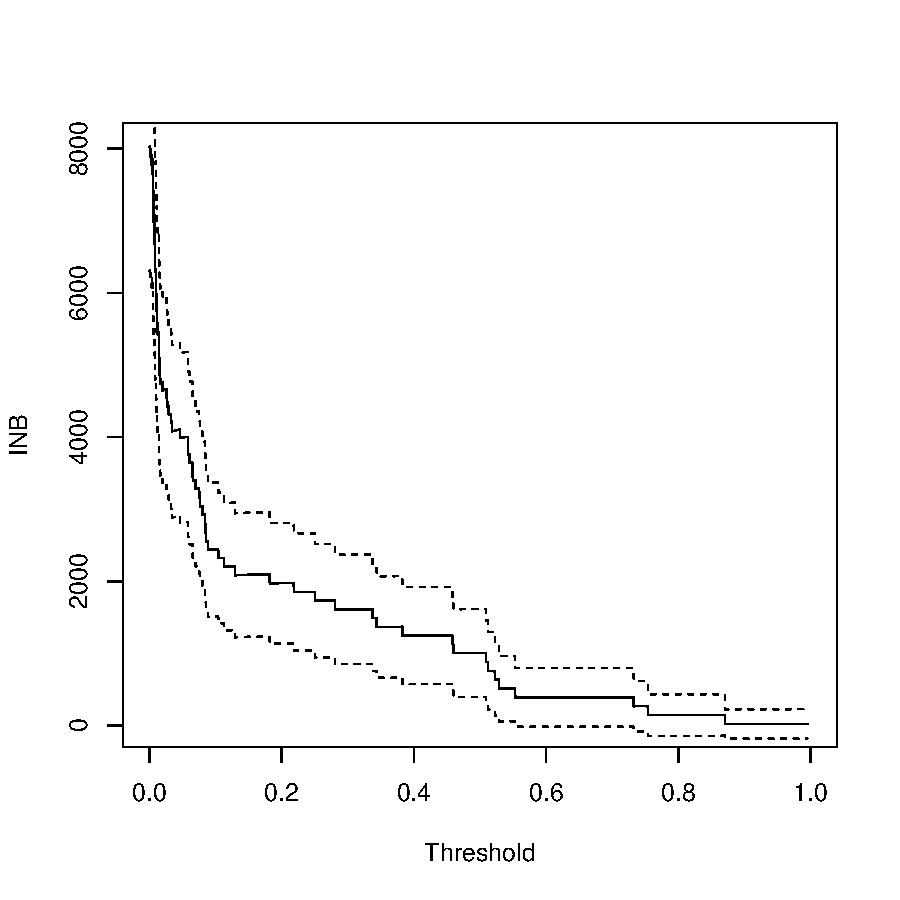
\includegraphics{Screening_biomarker_07142018-fig3}
\end{center}
\label{fig:three}
\caption{INB (solid line) with 95\% confidence intervals (dashed lines) for Ashkenazi-Jews.}
\end{figure}


Notice that a model-based estimator can be obtained as well by employing the joint model for $M$ and $D$ described in (\ref{expressions}), and statistical inference can be based on the asymptotic normality of the MLE.

\subsection{Sensitivity Analyses}

\subsubsection{With respect to input parameters}

It is common in cost-effectiveness to see how sensitive the results are (i.e., INB herein) with respect to changes in input parameters. The input parameters are the cost (i.e., $c_0$, $c_1$, $c_2$ and $c_m$)and the effectiveness (i.e., $e_1$ and $e_2$) parameters. Since INB is linear in these parameters and $P(D+,M+)$ and $P(M+)$ are assumed fixed, it is straightforward to assess the sensitivity of the results (e.g., assuming these cost and effectiveness input parameters are normally distributed yields a normally distributed INB).

\subsubsection{With respect to the risk-model}

\textcolor{blue}{\it Now that I look at it in this way, the model in Section 3 could be thought of as allowing for error in the risk-model (still unbiased, but with some random error), hence it is a sensitivity analysis. Could you please provide density plots for the risk marker $M$ in AJ and the general population? Separately, we want to see whether we could employ some parametric model.}

% \subsection{INB for testing no one or testing everyone}
% 
% Note $pi_{INB}$ finds the interior maximum for $INB(m_0)$.  The boundaries of testing no one and testing everyone have to be compared to $INB(\pi_{INB})$ to see which is greatest. If we test no one, then $INB=0$.  If we test everyone, we can set $c_m=0$ since we don't need the marker, and
% \begin{eqnarray*}
%   INB_{all} &=& [(e_1-e_2)-(c_1-c_2-c_0)]\pi - c_0\\
%             &=& [e+c_0]\pi - c_0, 
% \end{eqnarray*}
% and thus we have an intuitive form for INB:
% \begin{eqnarray*}
%   INB &=& (e+c_0)MRS/2 - c_m + p[e\pi + c_0\pi - c_0] \\
%       &=& (e+c_0)MRS/2 - c_m + pINB_{all}.
% \end{eqnarray*}
% 
% \subsection{Minimum MRS, and maximum marker cost, for using marker to beat testing no one}
% 
% For beating testing no one (INB=0), set the INB equation above to be greater than zero and solve for MRS:
% \begin{eqnarray*}
%   MRS &>& 2\frac{c_m-pINB_{all}}{e+c_0}
% \end{eqnarray*}
% The right side is maximized if $p=0$.  Thus the minimum MRS for the biomarker to beat testing no one is
% \begin{eqnarray*}
%   MRS_{min} &=& 2\frac{c_m}{e+c_0}.
% \end{eqnarray*}
% Marker cost is key for setting this minimum MRS, which only depends on utilities.  Recall that the maximum MRS for a disease is $2\pi(1-\pi)$.  This also sets a maximum marker cost, beyond which it is not cost-effective to use even a perfect test:
% \begin{eqnarray*}
%   c_m &\le& \pi(1-\pi)(e+c_0)
% \end{eqnarray*}
% 
% \subsection{Minimum MRS, and maximum marker cost, for using marker to beat testing everyone}
% 
% For beating testing everyone ($INB=INB_{all}$), set the INB equation above to be greater than $INB_{all}$ and solve for MRS:
% \begin{eqnarray*}
%   MRS &>& 2\frac{c_m+(1-p)INB_{all}}{e+c_0}
% \end{eqnarray*}
% For the biomarker to beat testing everyone,

\section{Generalizing to usual screening with entry criteria and screening test}

We have considering only 1 screening test applied to the entire population, with everyone screening positive getting the confirmatory test.  But usually the whole population is not considered for screening a priori, only subsets based on age and sex, or ideally, subsets with sufficient risk of disease.  Thus there are really two tests for even the simplest screening: the first test is the criteria for entry into screening, the second test is the usual biomarker screening test used to decide who should get the confirmatory test.  We call the first test the "rule-out" test $M_O$ as its main goal is to keep out those whom we are sure have no benefit from screening, and the second test the "rule-in" test $M_I$ as its goal is to find those who might have disease today and should get the confirmatory test (Castle and Katki, Nat Rev Clin Oncol 2016).  Thus we first see if a person is eligible for screening $M_O+$, then only those get the screening test $M_I$.  

All the notation of Section 1 applies, except that now there are separate costs for the screening tests $c_O$ and $c_I$.  I also use the notation $e_0$ for the effectiveness in those without disease, which is normal life-expectancy (this is denoted as "1" in Section 1).  

We again calculate the increase in effectiveness and cost due to screening versus no screening.  The "no screening" scenario remains the same:
\begin{enumerate}
	\item{The individual has cancer ($D+$): cost is $c_0+c_2$ and effectiveness is $e_2$}
	\item{The individual does not have cancer ($D-$): cost is 0, effectiveness is 1.}
\end{enumerate}

\noindent Now screening is a two-step "rule-out/rule-in" procedure:
\begin{enumerate}
	\item{We first apply marker $M_O$.  Those who test $M_O-$ are not eligible for screening, but the following outcomes occur for them:
		\begin{enumerate}
			\item{The individual has cancer ($D+$): cost is $c_O+c_0+c_2$ and effectiveness is $e_2$.  This has probability $P(D+,M_O-)$.}
			\item{The individual does not have cancer ($D-$): cost is $c_O$, effectiveness is $e_0$.  This has probability $P(D-,M_O-)$.}
	\end{enumerate}
	}
	\item{Those who are $M_O+$ now get $M_I$. There are four possibilities:
		\begin{enumerate}
			\item{The screening is positive and the individual has cancer ($M_I+,D+$): cost is $c_O+c_I+c_0+c_1$ and effectiveness is $e_1$.  This has probability $P(D+,M_I+,M_O+)$.}
			\item{The screening is positive but the individual does not have cancer ($M_I+,D-$): cost is $c_O+c_I+c_0$ and effectiveness is $e_0$.  This has probability $P(D-,M_I+,M_O+)$.}
			\item{The screening is negative but the individual has cancer ($M-,D+$): cost is $c_O+c_I+c_0+c_2$ and effectiveness is $e_2$.  This has probability $P(D+,M_I-,M_O+)$.}
			\item{The screening is negative and the individual does not have cancer ($M-,D-$): cost is $c_O+c_I$ and effectiveness is $e_0$.  This has probability $P(D-,M_I-,M_O+)$.}
		\end{enumerate}  
	}
\end{enumerate}

Let $C$ and $E$ denote the cost and effectiveness without screening:
\begin{eqnarray*}
	{\cal E} (C) &=& (c_0+c_2)\cdot P(D+) \\
	{\cal E} (E) &=& e_2\cdot P(D+) + P(D-)
\end{eqnarray*}

\noindent With "rule-in/rule-out" screening,the costs and effectiveness are
\begin{eqnarray*}
	{\cal E} (C_M) &=& c_O + P(M_O+)\cdot c_I + [P(D+)+P(D-,M_I+,M_O+)]\cdot c_0 \\
	               &&+[P(D+)-P(D+,M_I+,M_O+]\cdot c_2+P(D+,M_I+,M_O+)\cdot c_1\\
	{\cal E} (E_M) &=& P(D-)\cdot e_0 + P(D+,M_I+,M_O+)\cdot e_1 + [P(D+)-P(D+,M_I+,M_O+)]\cdot e_2 \,.
\end{eqnarray*}
Comparing to section 1 for a single test, the effectiveness has the same form: you only get early detection effectiveness $e_1$ if you are double-positive and have disease $(D+,M_I+,M_O+)$, and you get late detection effectiveness $e_2$ for all other cases of disease $P(D+)-P(D+,M_I+,M_O+)$.  Similarly, comparing to section 1 for a single test, the cost has the same form: everyone gets eligibility screen $c_O$, those who test positive $M_O+$ get the rule-in screen $c_I$, the confirmatory test $c_0$ is given to everyone with disease and the false-double-positives $P(D+)+P(D-,M_I+,M_O+)$, early-detection cost accrues only to those double-positive and with disease $P(D+,M_I+,M_O+)$, and late-detection cost accrues to everyone else with disease $P(D+)-P(D+,M_I+,M_O+)$.

The increase in effectiveness for screening versus not screening are:
\begin{eqnarray*}
	\Delta E &=& (e_1 - e_2)\cdot P(D+,M_I+,M_O+)\,.
\end{eqnarray*}
This is the same as in section 1 for a single test, but now the probability must include $M_O+$ to identify the only group that gets early-detection, which is the only group whose live can be extended by screening.

The increase in costs for screening versus not screening are:
\begin{eqnarray*}
	\Delta C &=& c_O + c_I\cdot P(M_O+) + c_0\cdot P(D-,M_I+,M_O+) + c_1\cdot P(D+,M_I+,M_O+) + c_2\cdot P(D-,M_I+,M_O+)\\
	         &=& c_O + c_I\cdot P(M_O+) + c_0\cdot P(M_I+,M_O+) + (c_1 - c_2 - c_0)\cdot P(D+,M_I+,M_O+)
\end{eqnarray*}
The intuition here is the same as for section 1 with a single test.  Screening has extra $c_O$ for everyone, extra $c_I$ for the screening-eligible ($M_O+$), an extra confirmatory test for the false-double-positives $(D-,M_I+,M_O+)$, early-detection cost for those with early-detected disease $(D+,M_I+,M_O+)$, and extra late-detection cost for the false-double-positives $(D-,M_I+,M_O+)$.  The final expression is the same as that in section 1 for a single test, except that we have to include the cost of the extra test among screening-eligibles and include $M_O+$ in the joint probabilities for the terms involving the confirmatory test and treatment costs.

The $INB=\Delta E-\Delta C$ is (denoting $e=(e_1-e_2)-(c_1-c_2)$)
\begin{eqnarray*}
INB &=& (e+c_0)\cdot P(D+,M_I+,M_O+) - c_O - c_I\cdot P(M_O+) - c_0\cdot P(M_I+,M_O+).
\end{eqnarray*}
This has the same form for INB for a single test, except it includes second test cost $c_I$ and includes $M_O$ in all joint probabilities.


\subsection{Optimal cutoff thresholds for general 1-time screen}

Here we try to derive expressions for the 2 thresholds required $M_O<m_O$ and $M_I<m_I$ to maximize the $INB=\Delta E - \Delta C$.  I may well have done this wrong and hope you can see a simple way to a solution.

As in the 1 marker case, I presume we have an unbiased risk calculator, this time involving both markers:
\begin{eqnarray*}
P(D+|M_I=m_I,M_O=m_O) = P(D+|R(m_I,m_O)=r(m_I,m_O)) = r(m_I,m_O).
\end{eqnarray*}
The annoying thing is that this time there is some function $r()$ rather than just unbiased risk estimates $m_I$ or $m_O$.  Maybe $r()$ is linear or multiplicative or something, but I think it has to be specified.

The INB in terms of integrals is
\begin{eqnarray*}
INB &=& (e+c_0)\int_{m_O}^{\infty}\int_{m_I}^{\infty} r(m,n)f(m,n)~dm~dn - c_O - c_I\int_{m_O}^{\infty} f(m)~dm - c_0\int_{m_O}^{\infty}\int_{m_I}^{\infty} f(m,n)~dm~dn
\end{eqnarray*}
Taking partial derivatives with respect to $m_I$ and $m_O$:
\begin{eqnarray*}
\frac{\partial INB}{\partial m_I} &=& -(e+c_0)\int_{m_O}^{\infty} r(m_I,n)f(m_I,n)~dn + c_0\int_{m_O}^{\infty} f(m_I,n)~dn\\
\frac{\partial INB}{\partial m_O} &=& -(e+c_0)\int_{m_I}^{\infty} r(m,m_O)f(m,m_O)~dm + c_If(m_O) + c_0\int_{m_I}^{\infty} f(m,m_O)~dm.
\end{eqnarray*}
Jointly setting these equal to zero and solving looks hard.  However, practical screening programs set the rule-in and rule-out thresholds separately rather than jointly.  So let's focus on the problem at hand in lung-cancer screening, which is, given that the thresholds for deciding a positive CT is set (i.e say $m_I$ is known), who should be eligible for screening (i.e. what is the optimal $m_O$)?  That means we only have $m_O$ to optimize:  
\begin{eqnarray*}
\frac{\partial INB}{\partial m_O} &=& -(e+c_0)f(m_O)\int_{m_I}^{\infty} r(m,m_O)f(m|m_O)~dm + c_If(m_O) + c_0f(m_O)\int_{m_I}^{\infty} f(m|m_O)~dm = 0\\
0 &=& -(e+c_0)\int_{m_I}^{\infty} r(m,m_O)f(m|m_O)~dm + c_I + c_0\int_{m_I}^{\infty} f(m|m_O)~dm.
\end{eqnarray*}
Writing this again in terms of probabilities
\begin{eqnarray*}
0 &=& -(e+c_0)P(D+|M_I+,M_O=m_O)P(M_I+|M_O=m_O) + c_I + c_0P(M_I+|M_O=m_O).
\end{eqnarray*}
I had thought that a second simplifying assumption would be based on the fact that the two thresholds are decided independently.  But that doesn't mean that $M_I\pm$ is independent of $M_O\pm$.  In fact, telling me that you are eligible for screening ought to increase the chance that you will test positive on the screening test.  So I'm left with this integral equation that I think requires specifying parametric forms for the probabilities to make further progress.


% 
% First, since $M_O$ and $M_I$ are unbiased risk-models, 
% \begin{eqnarray*}\label{risk_model}
% P(D+|M_O=m_O) &=& m_O  \\
% P(D+|M_I=m_I) &=& m_I \,.
% \end{eqnarray*}
% 
% Let $f_M$ denote the density of $M$, so that one obtains
% \begin{eqnarray} \nonumber
% P(M+) &=& \int_{m_0}^\infty f_M(m)\,dm\\  \label{expressions}
% P(D+,M+) &=& \int_{m_0}^\infty P(D+|M=m)\cdot f_M(m)\,dm\\   \nonumber
%          &=& \int_{m_0}^\infty m\cdot f_M(m)\,dm\,.
% \end{eqnarray}
% INB can be writen as 
% \begin{equation}\label{INB}
% INB = A\cdot P(D+,M+) - B\cdot P(M+) -C\,, 
% \end{equation}
% where $A=(e_1-e_2) - (c_1-c_2-c_0)$, $B=c_0$ and $C=c_m$.
% Replacing (\ref{expressions}) in (\ref{INB}) yields
% \begin{equation}\label{INB2}
% INB=A\cdot \int_{m_0}^\infty m\cdot f_M(m)\,dm - B\cdot \int_{m_0}^\infty f_M(m)\,dm - C\,.
% \end{equation}
% Taking derivative with respect to $m_0$ and setting it to zero yields
% \[-A\cdot m_0\cdot f_M(m_0) + B\cdot f_M(m_0) =0\,, \]
% so that INB is maximized at $m_0=B/A$. 
% 
% 
% One then selects $m_0$ based on both $\Delta C$ and $\Delta E$. Notice that $\Delta E$ is maximized when $m_0=-\infty$ (i.e., screen everybody). 
% 
% \subsection{Application to a single CT lung-cancer screen}
% 
% 
% We previously applied MRS to the controversy over who should get tested for mutations in the \textit{BRCA1/2} genes, which cause high risks of breast and ovarian cancer~\citep{katki}.  The mutations are rare in the general population ($\approx0.25\%$), but are 10 times more common among Ashkenazi-Jews~\citep{STRUEWING1997}.  Currently, according to the UK National Institute for Health and Care Excellence (NICE) and the US Preventive Services Task Force, women are referred for mutation testing only if they have a strong family history of breast or ovarian cancer~\citep{Moyer2014} as quantified by a risk model calculating that their risk of carrying a mutation exceeds 10\%~\citep{NICE2017}.  However, as mutation-testing costs fall, prominent voices have called for testing \textit{all} women~\citep{King2014,GenomeWeb2017}.  \textit{BRCA1/2} testing is already being offered to a large unselected Canadian population as a demonstration project~\citep{GenomeWeb2017a}.  Testing all women would strain clinical resources by testing millions of women, $99.75\%$ of whom will test negative.  At US \$500-\$1,000 per test, testing millions of women has clear commercial implications.  
% 
% In contrast, we recently demonstrated that 80\% of Ashkenazi-Jewish mutation-carriers could be identified by testing only 44\% of Ashkenazi-Jewish women~\citep{Best2017}.  This is achieved by a low mutation-risk threshold of 0.78\%, far lower than the current 10\% UK NICE and US recommendation.   However, we could not formally justify any choice of risk-threshold.  To better understand the implications of different choices of risk threshold, we previously considered multiple metrics, including AUC, Net Benefit, and MRS/NBI \citep{katki}.  We showed that risk thresholds between 0.78\% to 5.0\% maximized the MRS ($\approx 1.7\%$) for Ashkenazi-Jewish women, and for the general population, thresholds between 0.07\% to 0.56\% maximized the MRS ($\approx 0.18\%$)~\citep{katki}.  Here we compare risk thresholds that maximize MRS to risk thresholds that maximize the INB.
% 
% We use data on 4,589 volunteers (102 \textit{BRCA1/2} mutation carriers) from the Washington Ashkenazi Study (WAS)~\citep{STRUEWING1997}.  We calculated each volunteer's risk of carrying a mutation, based on their self-reported family-history of breast/ovarian cancers, using the BRCAPRO risk model~\citep{Parmigiani1998}.  Here $M$ is the BRCAPRO risk score, and because BRCAPRO is a well-calibrated risk model~\citep{Best2017}, $m_0=R$, i.e. the cutpoint $m_0$ equals the risk threshold $R$. Disease $D$ indicates the presence of a \textit{BRCA1/2} mutation.
% 
% \subsection{Costs and Effectiveness of \textit{BRCA1/2} genetic testing, preventive interventions, and cancer treatments}
% 
% Let us redefine Effectiveness as the dollar value of the life-years gained by undergoing genetic testing.  Let us presume that  women without mutations have a normal lifespan of age 80.  \textit{BRCA1/2} mutation-carriers have 5.7 fewer years of expected life~\citep{mai}, so we set their life-expectancy to age 74.  
% 
% If mutation-carriers get genetic testing, they will act to reduce their cancer risks.  Most mutation-carriers undergo oophorectomy, the removal of ovaries.  Some also choose to have mastectomy, the removal of breasts.  These surgeries reduce cancer risk drastically, but not entirely; there is typically a 10\% chance that cancer occurs in each organ anyway.  These women also undergo frequent screening, and if cancer is found early, hopefully treatment is more effective.  I don't know what their life-expectancy is, but let me set it as age 78.
% 
% I set the dollar-value of each life-year gained as \$100,000 per year.  Thus Effectiveness is
% \begin{eqnarray*}
% 	e_1-e_2 &=& (78-74)\times\$100,000 = \$400,000
% \end{eqnarray*}
% 
% For costs, $c_m$ is the cost of using the BRCAPRO risk model.  This is very low-cost, but you need to come to the doctor's office, your family history has to be elicited, it takes time.  I will set it to the cost of a doctor's visit, say \$100.
% 
% $c_0$ is the cost of the BRCA genetic test.  Prices are falling, it is now about \$1,000.
% 
% $c_1$ is the cost of interventions for BRCA mutation carrier found by screening.  Generally they will undergo risk-reducting interventions, at least oophorectomy and perhaps also mastectomy, and then frequent lifetime cancer screening.  But cancer can still occur, and those 25\% (\textcolor{blue}{\it should this be related to the 10\% mentioned above?}) who still get cancer incur cancer treatment costs.  For $c_2$, this is the cost of cancer treatment for mutation carriers who are not found until cancer is diagnosed.  All of them will require full cancer treatment.  I don't know how to specify $c_1,c_2$.  Let me set them both equal to \$100,000 for now.
% 
% Thus we have for Costs:
% \begin{eqnarray*}
% 	c_m &=& \$100 \\
% 	c_0 &=& \$1,000 \\
% 	c_1 &=& \$100,000 \\
% 	c_2 &=& \$100,000. \\
% \end{eqnarray*}
% 
% %At a future time, it may be worth decomposing $c_1$ into the cost for the risk-reducing interventions that everyone







\appendix 
\section*{Appendix}
\label{Appendix}

\section*{MRS is maximized when dichotomizing at disease prevalence}
\label{maxMRSNBIatPrevalence}

Recall that $MRS(m_0)=2J(m_0)\pi(1-\pi)$, where $J(m_0)$ is Youden's index calculated at cutpoint $m_0$.  MRS is maximized as a function of cutpoint $m_0$ when Youden's index $J(m_0)$ is maximized, which occurs when dichotomizing at disease prevalence: $P(D+|M=m_0)=P(D+)=\pi$.  To prove this we differentiate Youden's index as a function of $m_0$ 
\begin{eqnarray*}
	J(m_0) &=& \int_{m_0}^\infty P(M=m|D+)-P(M=m|D-)~dm
\end{eqnarray*}
with respect to the cutpoint $m_0$ using the Leibniz Integral Rule:
\begin{eqnarray*}
	\frac{dJ(m_0)}{dm_0} &=& P(M=m_0|D-)-P(M=m_0|D+).
\end{eqnarray*}
Setting the derivative equal to zero, and using Bayes' rule:
\begin{eqnarray*}
	\frac{P(D+|M=m_0)P(M=m_0)}{\pi} &=& \frac{P(D-|M=m_0)P(M=m_0)}{1-\pi}\\
	P(D+|M=m_0) &=& \pi
\end{eqnarray*}
Thus dichotomizing marker/model $M$ at $m_0$ at disease prevalence $\pi$ maximizes Youden's index and thus MRS.  Thus the "sweetspot" of risk-thresholds that maximize MRS will always include disease prevalence.  At this cutpoint, MRS equals Total Gain~\citep{bura2001binary}.

\end{document}


\begin{thebibliography}{99}

\bibitem{katki}
Katki, H.A.. Novel decision-theoretic and risk-stratification metrics of predictive performance: Application to deciding who should undergo genetic testing.  arXiv:1711.05686v1 [stat.ME].

\bibitem{mai}
Mai PL, Chatterjee N, Hartge P, Tucker M, Brody L, Struewing JP, Wacholder S.  Potential excess mortality in BRCA1/2 mutation carriers beyond breast, ovarian, prostate, and pancreatic cancers, and melanoma.  PLoS One. 2009;4(3):e4812.

	\bibitem[\protect\citeauthoryear{Antoniou, Pharoah, Smith, and Easton}{Antoniou
		et~al.}{2004}]{Antoniou2004}
	Antoniou, A., P.~P.~D. Pharoah, P.~Smith, and D.~Easton (2004, Oct).
	\newblock The {BOADICEA} model of genetic susceptibility to breast and ovarian
	cancer.
	\newblock {\em Br J Cancer\/}~{\em 91\/}(8), 1580--90.
	
	\bibitem[\protect\citeauthoryear{Baker, Cook, Vickers, and Kramer}{Baker
		et~al.}{2009}]{Baker2009a}
	Baker, S.~G., N.~R. Cook, A.~Vickers, and B.~S. Kramer (2009, October).
	\newblock Using relative utility curves to evaluate risk prediction.
	\newblock {\em Journal of the Royal Statistical Society. Series A, (Statistics
		in Society)\/}~{\em 172}, 729--748.
	
	\bibitem[\protect\citeauthoryear{Best, Tucker, Frone, Greene, Peters, and
		Katki}{Best et~al.}{2017}]{Best2017}
	Best, A.~F., M.~A. Tucker, M.~N. Frone, M.~H. Greene, J.~A. Peters, and H.~A.
	Katki (2017).
	\newblock To test or not to test: {S}election criteria for population-based
	{BRCA1/2} mutation screening.
	\newblock {\em Submitted\/}.
	
	\bibitem[\protect\citeauthoryear{Bura and Gastwirth}{Bura and
		Gastwirth}{2001}]{bura2001binary}
	Bura, E. and J.~L. Gastwirth (2001).
	\newblock The binary regression quantile plot: Assessing the importance of
	predictors in binary regression visually.
	\newblock {\em Biometrical Journal\/}~{\em 43\/}(1), 5--21.
	
	\bibitem[\protect\citeauthoryear{Cantor and Kattan}{Cantor and
		Kattan}{2000}]{Cantor2000}
	Cantor, S.~B. and M.~W. Kattan (2000).
	\newblock Determining the area under the {ROC} curve for a binary diagnostic
	test.
	\newblock {\em Med Decis Making\/}~{\em 20\/}(4), 468--470.
	
	\bibitem[\protect\citeauthoryear{Cook}{Cook}{2007}]{Cook2007}
	Cook, N.~R. (2007, Feb).
	\newblock Use and misuse of the receiver operating characteristic curve in risk
	prediction.
	\newblock {\em Circulation\/}~{\em 115\/}(7), 928--935.
	
	\bibitem[\protect\citeauthoryear{Copas}{Copas}{1999}]{Copas1999}
	Copas, J. (1999).
	\newblock The effectiveness of risk scores: The logit rank plot.
	\newblock {\em Journal of the Royal Statistical Society. Series C (Applied
		Statistics)\/}~{\em 48\/}(2), 165--183.
	
	\bibitem[\protect\citeauthoryear{Gail and Pfeiffer}{Gail and
		Pfeiffer}{2005}]{Gail2005}
	Gail, M.~H. and R.~M. Pfeiffer (2005, April).
	\newblock On criteria for evaluating models of absolute risk.
	\newblock {\em Biostatistics (Oxford, England)\/}~{\em 6}, 227--239.
	
	\bibitem[\protect\citeauthoryear{Greenhouse, Cornfield, and
		Homburger}{Greenhouse et~al.}{1950}]{GREENHOUSE1950}
	Greenhouse, S.~W., J.~Cornfield, and F.~Homburger (1950, Nov).
	\newblock The {Y}ouden index: letters to the editor.
	\newblock {\em Cancer\/}~{\em 3\/}(6), 1097--1101.
	
	\bibitem[\protect\citeauthoryear{Hanley and McNeil}{Hanley and
		McNeil}{1982}]{Hanley1982}
	Hanley, J.~A. and B.~J. McNeil (1982, April).
	\newblock The meaning and use of the area under a receiver operating
	characteristic ({ROC}) curve.
	\newblock {\em Radiology\/}~{\em 143}, 29--36.
	
	\bibitem[\protect\citeauthoryear{Hilden}{Hilden}{1991}]{Hilden1991}
	Hilden, J. (1991).
	\newblock The area under the {ROC} curve and its competitors.
	\newblock {\em Medical Decis Making\/}~{\em 11}, 95--101.
	
	\bibitem[\protect\citeauthoryear{Huang, Sullivan~Pepe, and Feng}{Huang
		et~al.}{2007}]{Huang2007}
	Huang, Y., M.~Sullivan~Pepe, and Z.~Feng (2007).
	\newblock Evaluating the predictiveness of a continuous marker.
	\newblock {\em Biometrics\/}~{\em 63\/}(4), 1181--1188.
	
	\bibitem[\protect\citeauthoryear{Katki}{Katki}{2006}]{Katki2005}
	Katki, H.~A. (2006, June).
	\newblock Effect of misreported family history on {M}endelian mutation
	prediction models.
	\newblock {\em Biometrics\/}~{\em 62\/}(2), 478--487.
	
	\bibitem[\protect\citeauthoryear{King, Levy-Lahad, and Lahad}{King
		et~al.}{2014}]{King2014}
	King, M.-C., E.~Levy-Lahad, and A.~Lahad (2014, September).
	\newblock Population-based screening for {BRCA1} and {BRCA2}: 2014 {L}asker
	{A}ward.
	\newblock {\em JAMA\/}~{\em 312}, 1091--1092.
	
	\bibitem[\protect\citeauthoryear{Kraemer}{Kraemer}{1992}]{Krae:eval:1992}
	Kraemer, H.~C. (1992).
	\newblock {\em Evaluating Medical Tests: Objective and Quantitative
		Guidelines}.
	\newblock Newbury Park, {CA}: Sage Publications Inc.
	
	\bibitem[\protect\citeauthoryear{Kraemer}{Kraemer}{2004}]{Kraemer2004}
	Kraemer, H.~C. (2004, Jan).
	\newblock Reconsidering the odds ratio as a measure of 2x2 association in a
	population.
	\newblock {\em Stat Med\/}~{\em 23\/}(2), 257--270.
	
	\bibitem[\protect\citeauthoryear{Kuchenbaecker, Hopper, Barnes, Phillips,
		Mooij, Roos-Blom, Jervis, van Leeuwen, Milne, Andrieu, Goldgar, Terry,
		Rookus, Easton, Antoniou, BRCA1, Consortium, McGuffog, Evans, Barrowdale,
		Frost, Adlard, Ong, Izatt, Tischkowitz, Eeles, Davidson, Hodgson, Ellis,
		Nogues, Lasset, Stoppa-Lyonnet, Fricker, Faivre, Berthet, Hooning, van~der
		Kolk, Kets, Adank, John, Chung, Andrulis, Southey, Daly, Buys, Osorio, Engel,
		Kast, Schmutzler, Caldes, Jakubowska, Simard, Friedlander, McLachlan,
		Machackova, Foretova, Tan, Singer, Olah, Gerdes, Arver, and
		Olsson}{Kuchenbaecker et~al.}{2017}]{Kuchenbaecker2017}
	Kuchenbaecker, K.~B., J.~L. Hopper, D.~R. Barnes, et~al. (2017, June).
	\newblock Risks of breast, ovarian, and contralateral breast cancer for {BRCA1}
	and {BRCA2} mutation carriers.
	\newblock {\em JAMA\/}~{\em 317}, 2402--2416.
	
	\bibitem[\protect\citeauthoryear{Lachin}{Lachin}{2000}]{Lac00}
	Lachin, J.~M. (2000).
	\newblock {\em Biostatistical Methods: The Assessment of Relative Risks}.
	\newblock New York: Wiley-Interscience.
	
	\bibitem[\protect\citeauthoryear{Moyer}{Moyer}{2014}]{Moyer2014}
	Moyer, V.~A. (2014, February).
	\newblock Risk assessment, genetic counseling, and genetic testing for
	{BRCA}-related cancer in women: {U.S.} {P}reventive {S}ervices {T}ask {F}orce
	recommendation statement.
	\newblock {\em Ann Int Med\/}~{\em 160}, 271--281.
	
	\bibitem[\protect\citeauthoryear{NICE}{NICE}{2017}]{NICE2017}
	NICE (2017).
	\newblock Familial breast cancer: classification, care and managing breast
	cancer and related risks in people with a family history of breast cancer,
	recommendation 1.5.11.
	\newblock Technical report, {National Institute for Health and Care Excellence}
	Clinical Guidance
	{https://www.nice.org.uk/guidance/cg164/chapter/Recommendations\#genetic-testing}.
	
	\bibitem[\protect\citeauthoryear{Parmigiani, Berry, and Aguilar}{Parmigiani
		et~al.}{1998}]{Parmigiani1998}
	Parmigiani, G., D.~Berry, and O.~Aguilar (1998, Jan).
	\newblock Determining carrier probabilities for breast cancer-susceptibility
	genes {BRCA}1 and {BRCA}2.
	\newblock {\em Am J Hum Genet\/}~{\em 62\/}(1), 145--158.
	
	\bibitem[\protect\citeauthoryear{Pauker and Kassirer}{Pauker and
		Kassirer}{1980}]{Pauker1980}
	Pauker, S.~G. and J.~P. Kassirer (1980, May).
	\newblock The threshold approach to clinical decision making.
	\newblock {\em N Engl J Med\/}~{\em 302\/}(20), 1109--1117.
	
	\bibitem[\protect\citeauthoryear{Pencina, D'Agostino, D'Agostino, and
		Vasan}{Pencina et~al.}{2008}]{Pencina2008}
	Pencina, M.~J., R.~B. D'Agostino, R.~B. D'Agostino, and R.~S. Vasan (2008,
	Jan).
	\newblock Evaluating the added predictive ability of a new marker: from area
	under the {ROC} curve to reclassification and beyond.
	\newblock {\em Stat Med\/}~{\em 27\/}(2), 157--72; discussion 207--12.
	
	\bibitem[\protect\citeauthoryear{Pepe, Janes, Longton, Leisenring, and
		Newcomb}{Pepe et~al.}{2004}]{Pepe2004}
	Pepe, M.~S., H.~Janes, G.~Longton, W.~Leisenring, and P.~Newcomb (2004, May).
	\newblock Limitations of the odds ratio in gauging the performance of a
	diagnostic, prognostic, or screening marker.
	\newblock {\em Am J Epidemiol\/}~{\em 159\/}(9), 882--890.
	
	\bibitem[\protect\citeauthoryear{Rizk}{Rizk}{2017}]{GenomeWeb2017}
	Rizk, C. (2017).
	\newblock Researchers debate merits of population-wide genetic testing at
	{AACR}.
	\newblock Technical report, {GenomeWeb}
	{https://www.genomeweb.com/genetic-research/researchers-debate-merits-population-wide-genetic-testing-aacr}.
	
	\bibitem[\protect\citeauthoryear{{Staff Reporter}}{{Staff
			Reporter}}{2017}]{GenomeWeb2017a}
	{Staff Reporter} (2017).
	\newblock {V}eritas {G}enetics to provide {BRCA} testing for {C}anadian
	hereditary cancer screening effort.
	\newblock Technical report, {GenomeWeb}
	{https://www.genomeweb.com/clinical-sequencing/veritas-genetics-provide-brca-testing-canadian-hereditary-cancer-screening}.
	
	\bibitem[\protect\citeauthoryear{Struewing, Hartge, Wacholder, Baker, Berlin,
		McAdams, Timmerman, Brody, and Tucker}{Struewing
		et~al.}{1997}]{STRUEWING1997}
	Struewing, J.~P., P.~Hartge, S.~Wacholder, S.~M. Baker, M.~Berlin, M.~McAdams,
	M.~M. Timmerman, L.~C. Brody, and M.~A. Tucker (1997).
	\newblock The risk of cancer associated with specific mutations of {BRCA1} and
	{BRCA2} among {A}shkenazi {J}ews.
	\newblock {\em N. Engl. J. Med.\/}~{\em 336}, 1401--1408.
	
	\bibitem[\protect\citeauthoryear{Sweeting and Thompson}{Sweeting and
		Thompson}{2012}]{Sweeting2012}
	Sweeting, M.~J. and S.~G. Thompson (2012, Apr).
	\newblock Making predictions from complex longitudinal data, with application
	to planning monitoring intervals in a national screening programme.
	\newblock {\em J R Stat Soc Ser A Stat Soc\/}~{\em 175\/}(2), 569--586.
	
	\bibitem[\protect\citeauthoryear{Vickers and Elkin}{Vickers and
		Elkin}{2006}]{Vickers2006}
	Vickers, A.~J. and E.~B. Elkin (2006).
	\newblock Decision curve analysis: a novel method for evaluating prediction
	models.
	\newblock {\em Med Decis Making\/}~{\em 26}, 565--574.
	
	\bibitem[\protect\citeauthoryear{Wentzensen and Wacholder}{Wentzensen and
		Wacholder}{2013}]{Wentzensen2013}
	Wentzensen, N. and S.~Wacholder (2013, Feb).
	\newblock From differences in means between cases and controls to risk
	stratification: a business plan for biomarker development.
	\newblock {\em Cancer Discov\/}~{\em 3\/}(2), 148--157.
	
	\bibitem[\protect\citeauthoryear{Youden}{Youden}{1950}]{YOUDEN1950}
	Youden, W.~J. (1950, Jan).
	\newblock Index for rating diagnostic tests.
	\newblock {\em Cancer\/}~{\em 3\/}(1), 32--35.

\end{thebibliography}


\end{document}

setwd("E://Staff/Ionut Bebu/METHODS/Optimal_Screening/Screening_Hormuzd/ANALYSIS")
%setwd("/Users/katkih/hkCurrent/Dropbox/RiskStratification/MRS/BRCA/code")

Sweave("Screening_biomarker.rnw",syntax="SweaveSyntaxNoweb")



